\section{Hypergeometric reduction and main result}
\label{sec:main_result}

With the type-2 solution in hand, we substitute \cref{eq:G-solution} into the equation for $\widehat S$. The result is a forced Riccati equation whose time dependence occurs only through $z_2/(1-z_2)$. We shift by a long-time root, linearise with the standard Riccati trick, change independent variable to $z_2$, match the Gauss hypergeometric equation, and fix the free mix of solutions by $\widehat S(0)=1$. The method is inspired by that of Antal and Krapivsky; the subsections below present each of the steps.


\begin{figure}[htbp]
  \centering
  
\includegraphics[width=\textwidth]{figures/fig08_derivation_pipeline/fig08.pdf}
  \captionsetup{labelformat=empty,labelsep=none}
  \caption{}
  \label{fig:derivation-pipeline}
\end{figure}

\subsection{Selecting the stable constant part}

As $\hat t\to\infty$, we have $\widehat G\to r_{2,-}$. With type~2 settled, the equation for $\widehat S$ becomes autonomous, so any long-time limit of $\widehat S$ must be a constant solution of the algebraic equation obtained by setting $\widehat S'=0$ with $\widehat G=r_{2,-}$. That constant is a long-time root of the limiting type-1 equation. Write
\begin{equation*}
\widehat S(\hat t)=X(\hat t)+h,
\end{equation*}
where $h$ is a constant still to be set and $X$ is the remaining time-dependent deviation from that plateau. Direct substitution into \cref{eq:S-scaled} gives
\begin{align*}
X'
={}&X^2+(2h-\hat\kappa_1)X
-\hat\nu\alpha_2\frac{z_2}{1-z_2}\\
&+\bigl[h^2-\hat\kappa_1h
+\hat\mu_1+\hat\nu r_{2,-}\bigr].
\end{align*}
We choose $h$ so that the final bracket vanishes. The resulting quadratic is
\begin{equation}
\label{eq:h-quadratic}
h^2-\hat\kappa_1h+\hat\mu_1+\hat\nu r_{2,-}=0,
\end{equation}
and we take the lower root
\begin{equation}
\label{eq:h-lower-root}
h=\frac{\hat\kappa_1-
\sqrt{\hat\kappa_1^2-4(\hat\mu_1+\hat\nu r_{2,-})}}{2}.
\end{equation}
With that choice, $h$ is exactly the long-time root: once $X\to0$, one has $\widehat S\to h$, which is the forever-avoidance probability from one initial type-1 individual. The coordinate $z_2$ is not needed to define $h$; only the settled value $r_{2,-}$ of $\widehat G$ enters \cref{eq:h-quadratic}.

We take the lower root because it is the stable attractor inside the admissible probability interval. Since $r_{2,-}\leq1$, the discriminant is bounded below by
\begin{align*}
\hat\kappa_1^2-4(\hat\mu_1+\hat\nu r_{2,-})
&\geq(1+\hat\mu_1+\hat\nu+\hat\delta_1)^2
-4(\hat\mu_1+\hat\nu)\\
&=(u-1)^2+2\hat\delta_1(1+u)+\hat\delta_1^2,
\end{align*}
where $u=\hat\mu_1+\hat\nu$, so the roots are real. Moreover
\[
2h-\hat\kappa_1
=-\sqrt{\hat\kappa_1^2-4(\hat\mu_1+\hat\nu r_{2,-})}<0,
\]
so the lower root is the stable attractor of the limiting autonomous equation, while the other root lies above one in the genuinely coupled catastrophe regime. With this choice, $X=\widehat S-h$ satisfies
\begin{equation}
\label{eq:X-riccati}
X'=X^2+(2h-\hat\kappa_1)X
-\hat\nu\alpha_2\frac{z_2}{1-z_2}.
\end{equation}

\subsection{Linearising the Riccati equation}
\label{sec:linearising}

We now want a linear equation. A Riccati equation of the form $X'=X^2+\cdots$ linearises under the standard Riccati trick $X=-(\log Z)'$ \cite{BenderOrszag1978}. Set
\begin{equation}
\label{eq:riccati-substitution}
X=-\frac{Z'}{Z}.
\end{equation}
Then
\[
X'=-\frac{Z''}{Z}+\left(\frac{Z'}{Z}\right)^2
=-\frac{Z''}{Z}+X^2.
\]
The quadratic terms cancel in \cref{eq:X-riccati}, and we land on the linear second-order equation
\begin{equation}
\label{eq:Z-linear}
Z''+(\hat\kappa_1-2h)Z'
-\hat\nu\alpha_2\frac{z_2(\hat t)}{1-z_2(\hat t)}Z=0,
\end{equation}
in which the only remaining awkwardness is the time-dependent coefficient of $Z$. Because $X$ depends on $Z$ only through the logarithmic derivative $Z'/Z$, any overall multiplicative constant in $Z$ cancels from the probability.

\subsubsection{Change of independent variable}

All remaining time dependence in \cref{eq:Z-linear} sits inside $z_2(\hat t)$: the coefficient is $z_2/(1-z_2)$, and $z_2$ itself is a known exponential function of $\hat t$. Measuring ``time'' by $z_2$ rather than by $\hat t$ turns a linear ODE with exponential-looking coefficients into the Gauss hypergeometric equation, whose solutions are known.

Since $z_2'=\hat q_2z_2$ and $z_2$ is monotone, write
\begin{equation*}
Z(\hat t)=\Phi(z_2(\hat t)).
\end{equation*}
If primes on $\Phi$ mean differentiation with respect to $z_2$, the chain rule gives
\begin{equation}
\label{eq:chain-Z}
Z'=\hat q_2z_2\Phi',
\end{equation}
and then
\begin{equation}
\label{eq:chain-Z2}
Z''=\hat q_2^2\bigl(z_2^2\Phi''+z_2\Phi'\bigr).
\end{equation}
Substitute \cref{eq:chain-Z,eq:chain-Z2} into \cref{eq:Z-linear}. For every finite $\hat t$, $z_2\neq0$, so we may divide by $\hat q_2^2z_2$ and obtain the intermediate form
\begin{equation*}
z_2\Phi''+\left(1+\frac{\hat\kappa_1-2h}{\hat q_2}\right)\Phi'
-\frac{\hat\nu\alpha_2}{\hat q_2^2}\frac{1}{1-z_2}\Phi=0.
\end{equation*}
Multiplying through by $(1-z_2)$ clears the remaining denominator and yields
\begin{equation}
\label{eq:hypergeometric}
z_2(1-z_2)\Phi''+C(1-z_2)\Phi'
-\frac{\hat\nu\alpha_2}{\hat q_2^2}\Phi=0,
\end{equation}
where
\begin{equation}
\label{eq:C-generalized}
C=1+\frac{\hat\kappa_1-2h}{\hat q_2}.
\end{equation}
Because $\hat q_2=-\hat\Delta_2$ and $\hat\kappa_1-2h>0$, this parameter always satisfies
\begin{equation*}
C=1-\frac{\hat\kappa_1-2h}{\hat\Delta_2}<1.
\end{equation*}

\subsubsection{Matching to the Gauss equation}

Equation \eqref{eq:hypergeometric} is an instance of the canonical Gauss hypergeometric equation
\begin{equation*}
z(1-z)\Phi''+[C-(A+B+1)z]\Phi'-AB\Phi=0.
\end{equation*}
When $C\notin\mathbb Z$, its standard fundamental solutions are
\begin{subequations}
\label{eq:gauss-canonical-solutions}
\begin{align}
\Phi_1(z)&={}_2F_1(A,B;C;z),\\
\Phi_2(z)&=z^{1-C}
{}_2F_1(A-C+1,B-C+1;2-C;z).
\end{align}
\end{subequations}
Every solution is then a linear combination $\Phi=c_1\Phi_1+c_2\Phi_2$. The parameters $A$, $B$, and $C$ are fixed by matching coefficients with \cref{eq:hypergeometric}. Comparing the coefficient of $\Phi'$ already gave $C$ in \cref{eq:C-generalized}. The remaining matches are
\begin{equation}
\label{eq:ABC-relations}
A+B=C-1=\frac{\hat\kappa_1-2h}{\hat q_2},
\qquad
AB=\frac{\hat\nu\alpha_2}{\hat q_2^2}.
\end{equation}
Thus $A$ and $B$ are the two roots of one quadratic:
\begin{equation}
\label{eq:AB-explicit}
A,B=\frac{C-1}{2}\mathbin{\pm}
\sqrt{\frac{(C-1)^2}{4}
-\frac{\hat\nu\alpha_2}{\hat q_2^2}}.
\end{equation}
They need not be individually real. If the discriminant is negative, they form a complex-conjugate pair; the differential equation and its physical boundary data remain real. At this point the differential equation for $\Phi$ is completely specified. What remains is to rebuild the probability and fix the free mix of the two solutions.

\subsection{The closed formula}
\label{sec:closed-formula}

\subsubsection{Rebuilding $\widehat S$ from $\Phi$}

We first reverse the substitutions, before choosing a basis for $\Phi$. From
\[
\widehat S=h+X,
\qquad
X=-\frac{Z'}{Z},
\qquad
Z=\Phi(z_2),
\]
the chain rule \cref{eq:chain-Z} gives
\begin{equation}
\label{eq:S-from-Phi}
\widehat S(\hat t)
=h-\hat q_2z_2(\hat t)
\frac{\Phi'(z_2(\hat t))}{\Phi(z_2(\hat t))}.
\end{equation}
The probability depends on $\Phi$ only through the logarithmic derivative $\Phi'/\Phi$. Any overall multiplicative constant in $\Phi$ cancels, as already noted for $Z$.

\subsubsection{Ansatz for $\Phi$: the two-dimensional solution space}

Equation \eqref{eq:hypergeometric} is a second-order linear ODE, so its solution space is two-dimensional. We do not guess $\Phi$ as a special function of the probability; we take the general solution of the equation we have derived. For $C\notin\mathbb Z$ that general solution is any mix of the standard pair \cref{eq:gauss-canonical-solutions}.

Our path has $z_2(\hat t)<0$ for all finite $\hat t$, so we evaluate everything on the negative real axis. The textbook second solution uses the factor $z^{1-C}$, which need not stay real for $z<0$ and real non-integer $C$. On the same path, $-z>0$, so we replace that factor by $(-z)^{1-C}$ and work with the real-axis pair
\begin{subequations}
\label{eq:UV-definitions}
\begin{align}
U(z)&={}_2F_1(A,B;C;z),\\
V(z)&=(-z)^{1-C}
{}_2F_1(A-C+1,B-C+1;2-C;z).
\end{align}
\end{subequations}
Here $U$ is exactly $\Phi_1$, while $V$ plays the role of $\Phi_2$ in a form that stays real for real $C$ whenever $-z>0$. Thus $U$ and $V$ are two independent real solutions of the hypergeometric ODE on the negative axis where $z_2$ lives. Any solution $\Phi$ is a mix of them,
\begin{equation*}
\Phi(z)=c_1U(z)+c_2V(z),
\end{equation*}
with two coefficients $c_1,c_2$. Integer $C$ does not change that strategy; it only changes how one writes the second basis function (a logarithm may appear), as discussed in \cref{app:hypergeometric-details}.

Physics fixes only the mix of the two solutions, not the overall scale of $\Phi$. From \cref{eq:S-from-Phi}, $\widehat S$ depends on $\Phi$ only through $\Phi'/\Phi$. Scaling both coefficients by the same nonzero factor,
\[
(c_1,c_2)\longmapsto(\lambda c_1,\lambda c_2),
\]
leaves $\Phi'/\Phi$ unchanged, and therefore leaves $\widehat S$ unchanged. The overall scale of $\Phi$ is free: we never need absolute values of both coefficients. What we do need is the right \emph{mix}, equivalently the ratio $c_2/c_1$.

\subsubsection{Initial condition and the constant $L$}

That mix is fixed by the single initial condition $\widehat S(0)=1$. At $\hat t=0$ we have $z_2=z_{2,0}$. Inserting $\widehat S(0)=1$ into \cref{eq:S-from-Phi} gives
\[
1=h-\hat q_2z_{2,0}\frac{\Phi'(z_{2,0})}{\Phi(z_{2,0})},
\]
and therefore
\begin{equation}
\label{eq:L-definition}
\frac{\Phi'(z_{2,0})}{\Phi(z_{2,0})}
=L,
\qquad
L=\frac{h-1}{\hat q_2z_{2,0}}.
\end{equation}
There is only one physical condition on $\Phi$: its logarithmic derivative at the starting point $z_{2,0}$ must equal the number $L$. There is not a second condition that pins down $c_1$ and $c_2$ separately.

\subsubsection{Choosing the mix: coefficients $K_U$ and $K_V$}

It remains only to pick one concrete mix that satisfies \cref{eq:L-definition}. We write the same linear combination with names $K_U,K_V$ instead of $c_1,c_2$:
\begin{equation}
\label{eq:Phi-linear-combination}
\Phi(z)=K_U U(z)+K_V V(z).
\end{equation}
These are simply a particular choice of $(c_1,c_2)$, not new unknowns. Write
\begin{equation*}
U_0=U(z_{2,0}),
\quad
V_0=V(z_{2,0}),
\quad
U_0'=U'(z_{2,0}),
\quad
V_0'=V'(z_{2,0})
\end{equation*}
for the basis values at the initial coordinate. We take a convenient Wronskian normalisation,
\begin{subequations}
\label{eq:K-coefficients}
\begin{align}
K_U&=V_0'-L V_0,\\
K_V&=L U_0-U_0'.
\end{align}
\end{subequations}
This is a standard trick for a linear second-order equation. Once a fundamental pair is fixed, the two coefficients above are chosen so that $\Phi'/\Phi=L$ at $z_{2,0}$; multiplying both by the same nonzero constant does not change $\Phi'/\Phi$, so the overall scale of $(K_U,K_V)$ is free. Only the origin of $L$ is model-specific. At that point one has
\begin{equation*}
\Phi(z_{2,0})=U_0V_0'-U_0'V_0,
\qquad
\Phi'(z_{2,0})=L(U_0V_0'-U_0'V_0).
\end{equation*}
The common factor is the Wronskian of $(U,V)$ at $z_{2,0}$, which is nonzero for $C\notin\mathbb Z$. Hence $\Phi(z_{2,0})\neq0$ and $\Phi'(z_{2,0})/\Phi(z_{2,0})=L$ holds at once. Any other multiple $(\lambda K_U,\lambda K_V)$ would work equally well for $\widehat S$; the formulae above just pick one scale for us, without hand-solving for a ratio.

The same mix may equally be written $\Phi=U+D V$ with a single ratio
\begin{equation*}
D=\frac{K_V}{K_U}
=\frac{L U_0-U_0'}{V_0'-L V_0},
\end{equation*}
whenever $K_U\neq0$. In the present probability regime that is automatic: a pure-$V$ solution would tend, as $z\to0^-$, to a value strictly larger than one, contradicting $\widehat S\leq1$ from \cref{prop:feynman-kac}.


\subsubsection{Main formula}

\begin{theorem}[Exact finite-time no-catastrophe probability]
\label{tt:thm:main}
Assume $\lambda_1>0$, $\hat\lambda_2>0$, $\hat\delta_2>0$, $\hat\nu>0$, and $C\notin\mathbb Z$. With the quantities of this section defined as above, then
\begin{equation}
\boxed{
\widehat S(\hat t)=h-
\hat q_2z_2(\hat t)
\frac{K_U U'(z_2(\hat t))+K_V V'(z_2(\hat t))}
{K_U U(z_2(\hat t))+K_V V(z_2(\hat t))}}
\label{eq:S-final}
\end{equation}
solves \cref{eq:S-scaled} with $\widehat S(0)=1$. Together with \cref{eq:G-solution}, it gives both finite-time no-catastrophe probabilities. In physical time, after every hatted rate is replaced by the ratio in \cref{eq:scaled-rates},
\begin{equation}
\label{eq:unscaled-recovery}
\begin{aligned}
S(t)&=h-
\hat q_2z_2(\lambda_1t)
\frac{K_U U'(z_2(\lambda_1t))+K_V V'(z_2(\lambda_1t))}
{K_U U(z_2(\lambda_1t))+K_V V(z_2(\lambda_1t))},\\
G(t)&=r_{2,-}-\alpha_2\frac{z_2(\lambda_1t)}{1-z_2(\lambda_1t)}.
\end{aligned}
\end{equation}
A compact nested evaluation map for every constant appears later in this section (\cref{note:parameter-map}).
\end{theorem}

% \begin{proof}
% The shift by $h$ transforms \cref{eq:S-scaled} into \cref{eq:X-riccati}. The logarithmic derivative in \cref{eq:riccati-substitution} then gives \cref{eq:Z-linear}, and the coordinate $z_2$ gives the Gauss equation \eqref{eq:hypergeometric}. Relations \cref{eq:ABC-relations} identify its two parameters. The Wronskian construction in \cref{eq:K-coefficients,eq:Phi-linear-combination} imposes the initial logarithmic derivative \cref{eq:L-definition}, and substitution back through \cref{eq:S-from-Phi} yields \cref{eq:S-final}. Each change is reversible on a finite real interval because $z_2<0$ and the physical linearising function can be normalised as
% \[
% Z(\hat t)=Z(0)\exp\!\left\{-\int_0^{\hat t}X(s)\,\dd s\right\},
% \]
% which is nonzero whenever the Riccati solution is finite. Finally \cref{eq:unscaled-recovery} reverses the time scaling.
% \end{proof}

As $\hat t\to\infty$, one has $z_2\to0$ and therefore $\widehat G\to r_{2,-}$ and $\widehat S\to h$. These limits are the probabilities of avoiding catastrophe forever from one initial type-2 or type-1 individual, respectively. Checks of the initial slopes and degenerate parameter boundaries are collected in \cref{app:limits}.

The same result can be written as a logarithmic derivative,
\begin{equation*}
\widehat S(\hat t)=h-
\hat q_2z_2(\hat t)
\left.\frac{\dd}{\dd z}
\log\Phi(z)\right|_{z=z_2(\hat t)}.
\end{equation*}
This compact form exposes the Riccati structure.

\begin{remark}[A one-basis special case]
If the initial condition happens to give $K_V=0$, equivalently $D=0$, the theorem reduces to
\begin{equation*}
\widehat S(\hat t)
=h-\hat q_2z_2(\hat t)\frac{AB}{C}
\frac{{}_2F_1(A+1,B+1;C+1;z_2(\hat t))}
{{}_2F_1(A,B;C;z_2(\hat t))}.
\end{equation*}
\end{remark}

\Cref{fig:bdc-survival,fig:bdc-density} illustrate the closed formulae for a single rate vector: the no-catastrophe probabilities $S$ and $G$, and the corresponding defective catastrophe-time densities $-S'$ and $-G'$. The solid curves are the exact expressions of \cref{tt:thm:main}; open markers are an independent numerical check of the backward ODEs by classical fourth-order Runge--Kutta (RK4).

\begin{figure}[!htbp]
  \centering
  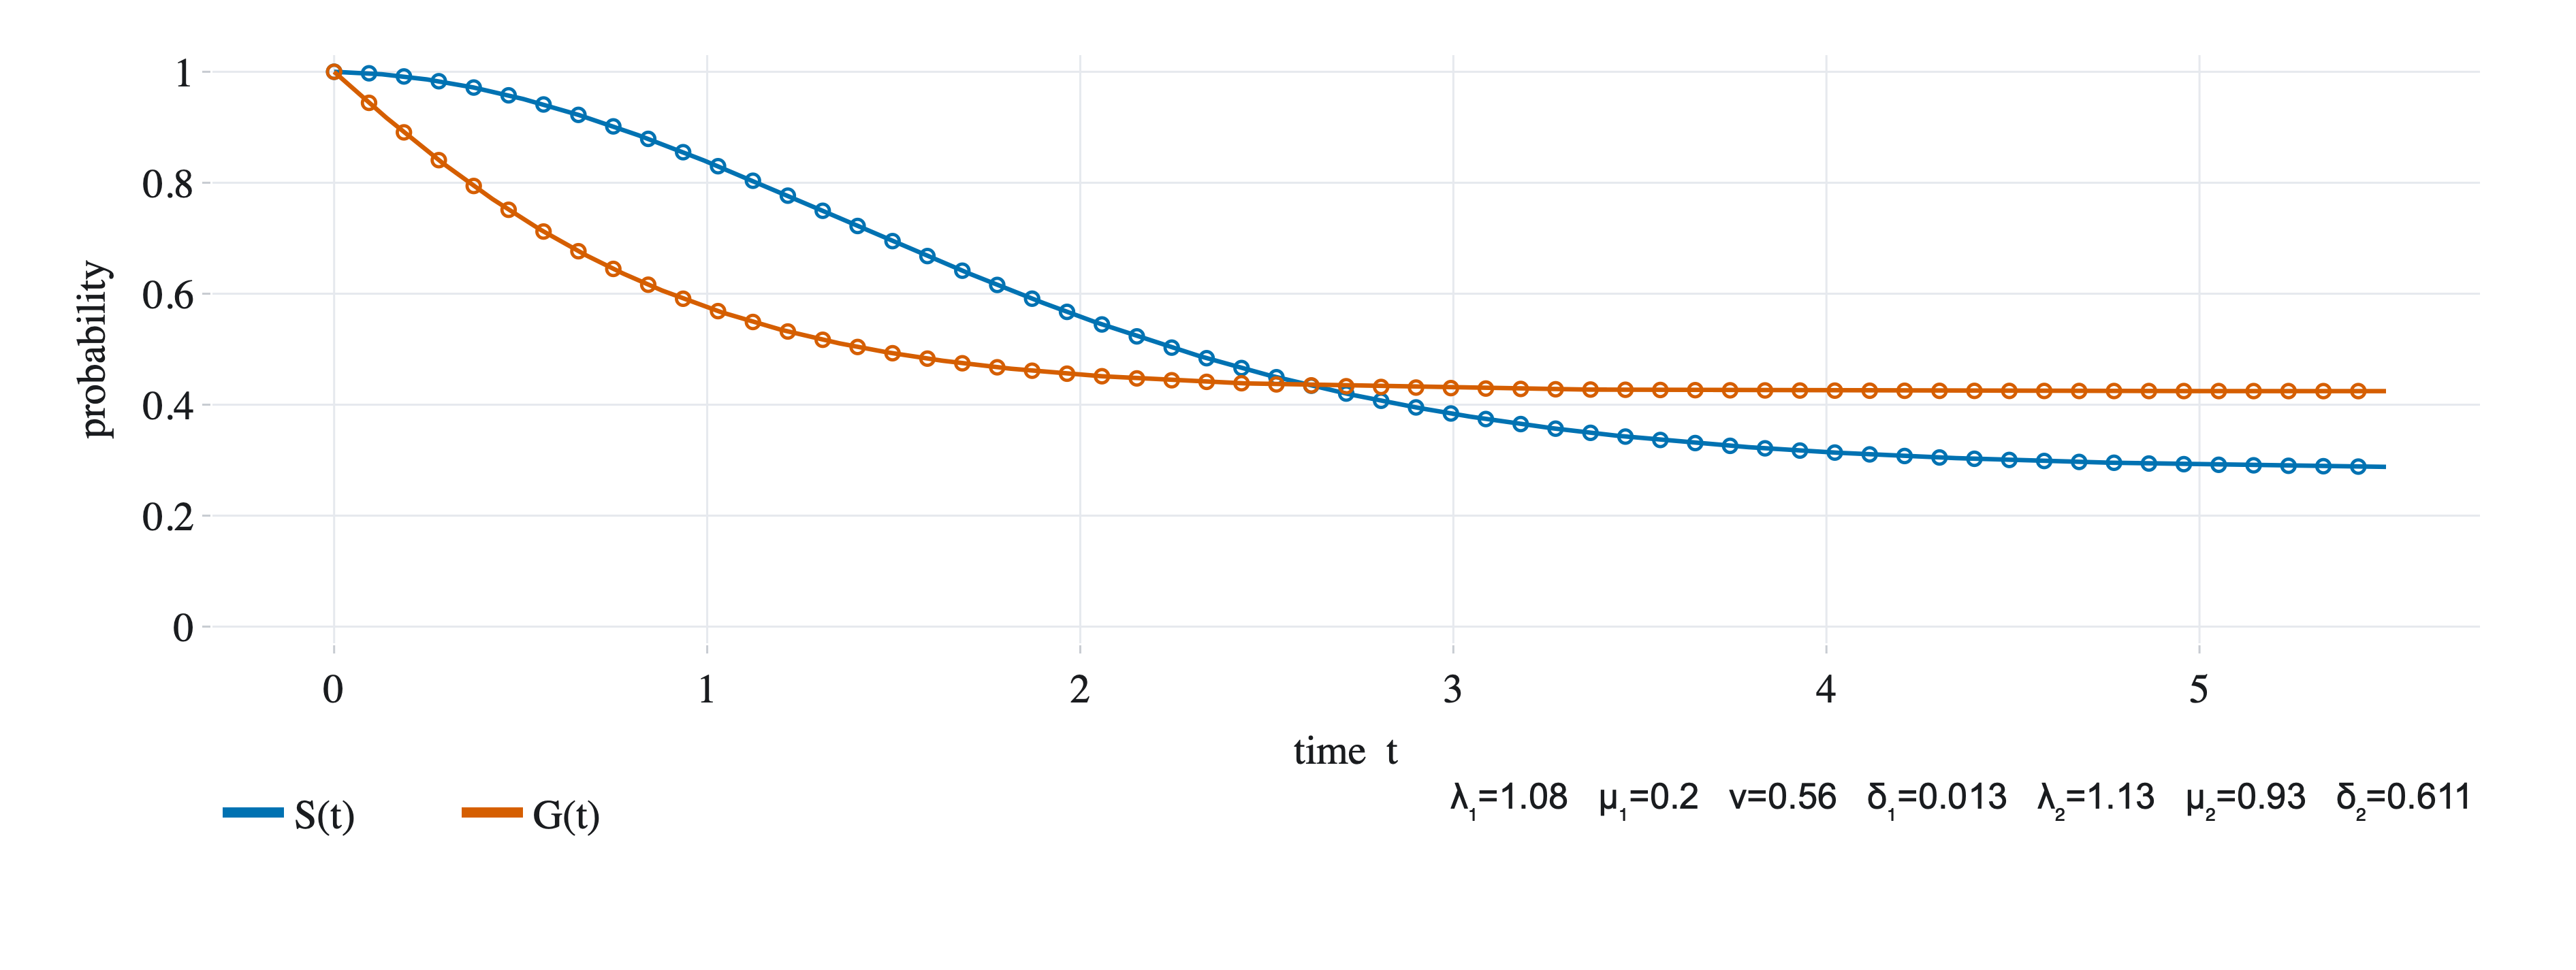
\includegraphics[width=\textwidth]{figures/fig_bdc_survival/panel_survival.png}
  \caption{No-catastrophe probabilities $S(t)$ (type~1 start) and $G(t)$ (type~2 start) at fixed rates
    $\lambda_1=1.08$, $\mu_1=0.2$, $\nu=0.56$, $\delta_1=0.013$,
    $\lambda_2=1.13$, $\mu_2=0.93$, $\delta_2=0.611$.
    Asymptotic levels $h=\lim S$ and $r_{2,-}=\lim G$ are indicated on the panel.
    Solid curves: closed form of \cref{tt:thm:main}; open circles: RK4 integration of the unscaled backward ODEs.
    Rates are labelled on the panel.
    \explorerlink{https://files.volvox.site/users/pages/6a6852d29e3764e44c80325e/files/1785222252388-TT_bdc_survival_visualiser.html}{Survival visualiser}}
  \label{fig:bdc-survival}
\end{figure}

\begin{figure}[!htbp]
  \centering
  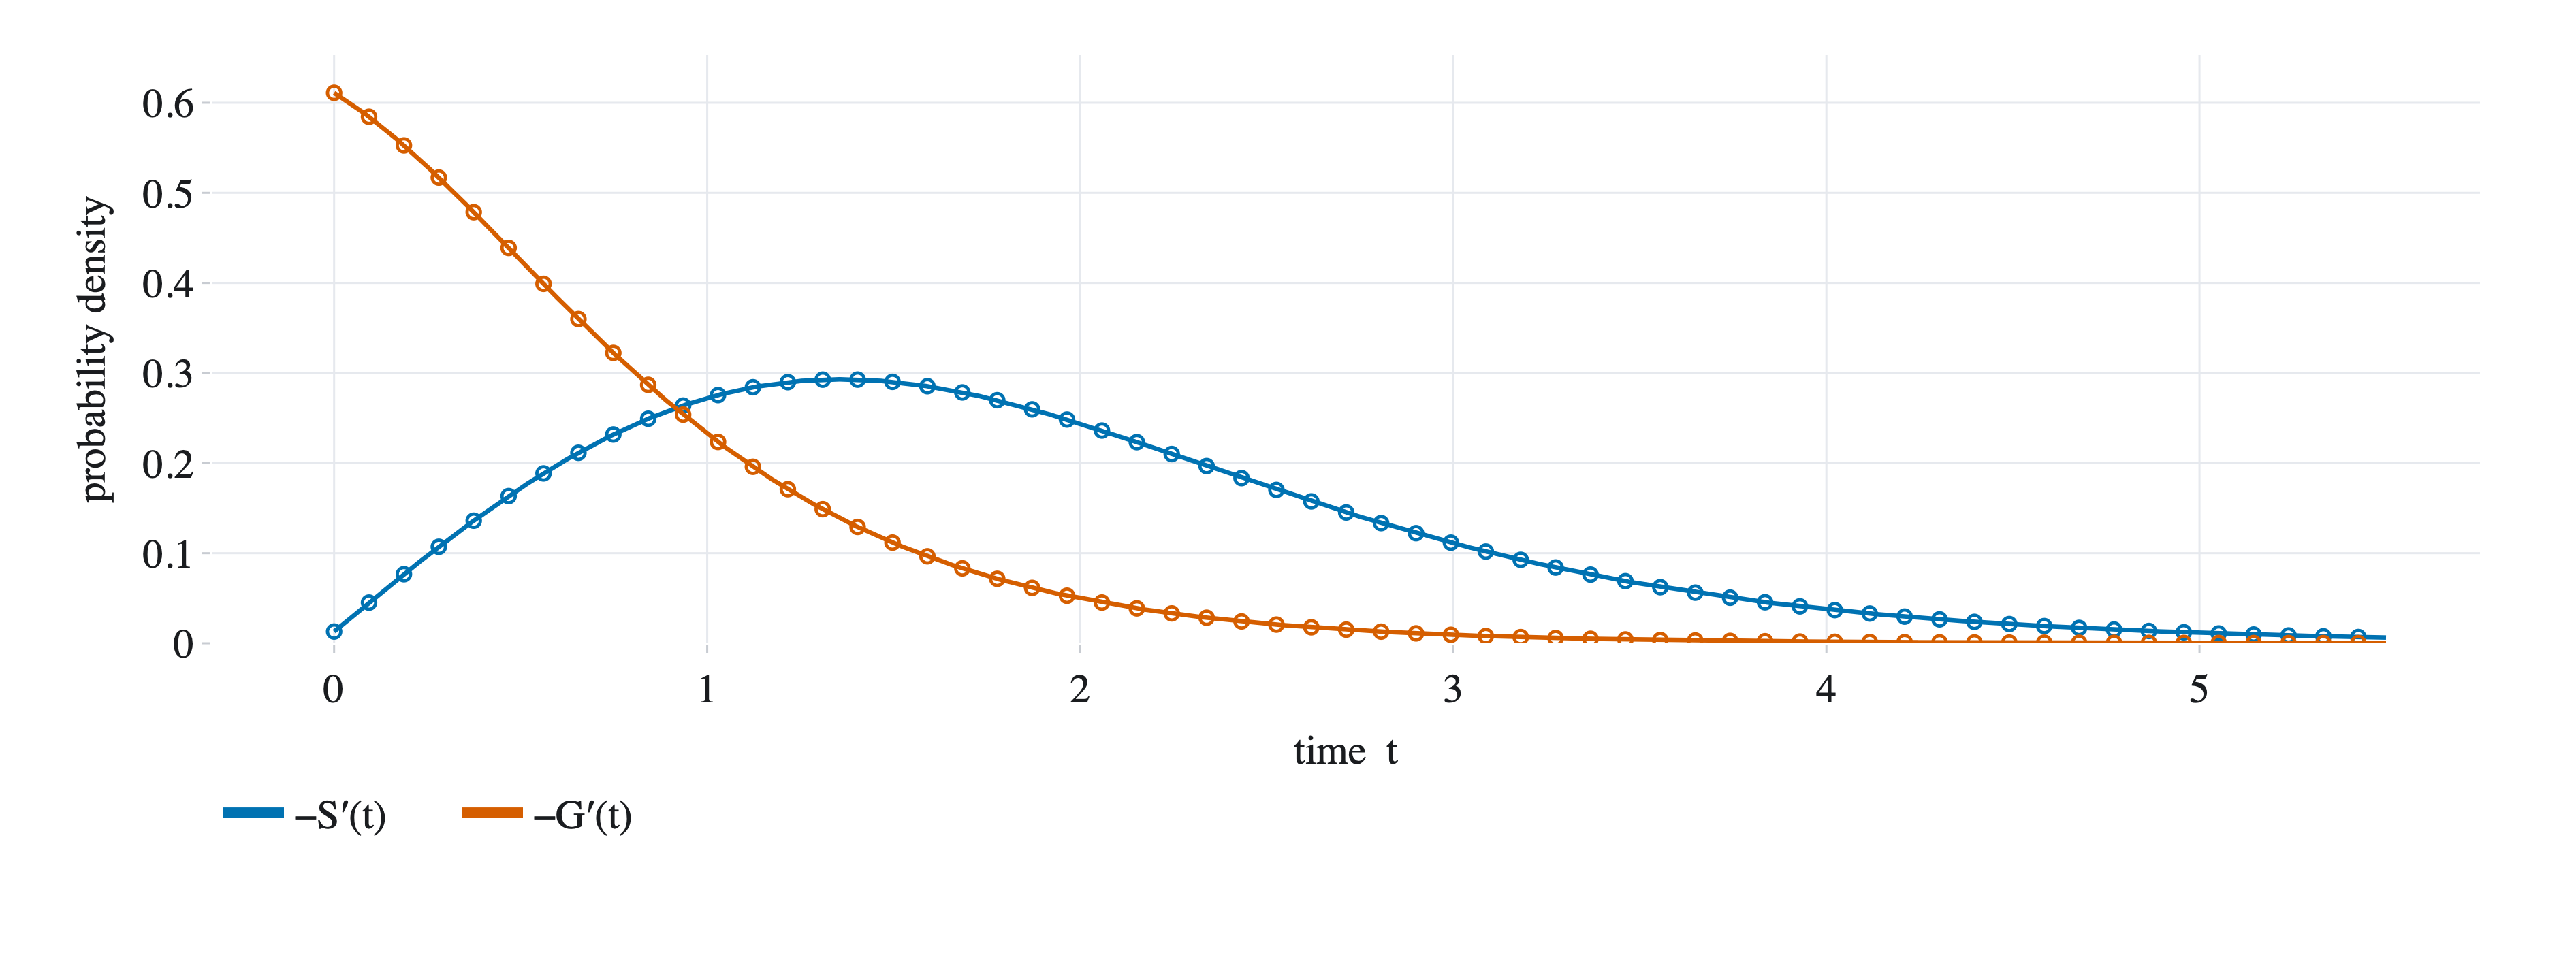
\includegraphics[width=\textwidth]{figures/fig_bdc_survival/panel_density.png}
  \caption{Defective catastrophe-time densities $-S'(t)$ and $-G'(t)$ for the same rates as \cref{fig:bdc-survival}.
    Solid curves from the closed form; open circles from the same RK4 check of the backward ODEs.}
  \label{fig:bdc-density}
\end{figure}

\FloatBarrier

\begin{remark}[Nested parameters]
\label{note:parameter-map}
Here every constant in \cref{eq:S-final,eq:unscaled-recovery} is fixed by the rates as follows. The real hypergeometric basis on the path $z_2<0$ is
\begin{equation*}
\begin{aligned}
U(z)&={}_2F_1(A,B;C;z),\\
V(z)&=(-z)^{1-C}
{}_2F_1(A-C+1,B-C+1;2-C;z).
\end{aligned}
\end{equation*}
The Wronskian mix enforcing $\widehat S(0)=1$ is then
\begin{equation*}
K_U=V_0'-L V_0,
\qquad
K_V=L U_0-U_0',
\end{equation*}
where $U_0=U(z_{2,0})$, $V_0=V(z_{2,0})$, $U_0'=U'(z_{2,0})$, $V_0'=V'(z_{2,0})$, and $L=(h-1)/(\hat q_2z_{2,0})$ is the required logarithmic derivative of $\Phi$ at $z_{2,0}$. The hypergeometric parameters are
\begin{equation*}
A,B
=\frac{C-1}{2}\mathbin{\pm}
\sqrt{\frac{(C-1)^2}{4}
-\frac{\hat\nu\alpha_2}{\hat q_2^2}},
\qquad
C=1+\frac{\hat\kappa_1-2h}{\hat q_2}.
\end{equation*}
The long-time root and type-1 coefficient are
\begin{equation*}
h=\frac{\hat\kappa_1
-\sqrt{\hat\kappa_1^2-4(\hat\mu_1+\hat\nu r_{2,-})}}{2},
\qquad
\hat\kappa_1=1+\hat\mu_1+\hat\nu+\hat\delta_1.
\end{equation*}
The type-2 coordinate and its ingredients are
\begin{equation*}
z_2(\lambda_1t)=z_{2,0}\e^{\hat q_2\lambda_1t},
\qquad
z_{2,0}=\frac{r_{2,-}-1}{r_{2,+}-1},
\qquad
\hat q_2=-\hat\Delta_2,
\qquad
\alpha_2=\frac{\hat\Delta_2}{\hat\lambda_2},
\end{equation*}
\begin{equation*}
r_{2,\pm}
=\frac{\hat\lambda_2+\hat\mu_2+\hat\delta_2\pm\hat\Delta_2}{2\hat\lambda_2},
\qquad
\hat\Delta_2
=\sqrt{(\hat\lambda_2+\hat\mu_2+\hat\delta_2)^2-4\hat\lambda_2\hat\mu_2}.
\end{equation*}
Finally the hatted rates are the original rates scaled by the type-1 birth rate,
\begin{equation*}
\hat\mu_i=\frac{\mu_i}{\lambda_1},
\qquad
\hat\nu=\frac{\nu}{\lambda_1},
\qquad
\hat\delta_i=\frac{\delta_i}{\lambda_1},
\qquad
\hat\lambda_2=\frac{\lambda_2}{\lambda_1}
\qquad(i=1,2),
\end{equation*}
so the formulae are completely determined by $(\lambda_1,\mu_1,\nu,\delta_1,\lambda_2,\mu_2,\delta_2)$ and the time $t$. Explicit derivatives of $U$ and $V$ are recorded in \cref{app:hypergeometric-details}.
\end{remark}

\subsection{Mathematical interpretation}
\label{sec:interpretation}

The formula in \cref{eq:S-final} is exact within the model: it is the finite-time no-catastrophe probability and, by \cref{prop:feynman-kac}, the occupation-time average of $\exp\bigl(-\delta_1\int X-\delta_2\int Y\bigr)$. The two catastrophe rates do not enter symmetrically. The type-2 rate $\hat\delta_2$ reshapes the roots $r_{2,\pm}$, the coordinate $z_2$, and the whole function $\widehat G$, which then drives the type-1 equation; the type-1 rate $\hat\delta_1$ enters only through $\hat\kappa_1$, so it changes $h$ and the hypergeometric parameters $A,B,C$ without feeding back into $\widehat G$. That asymmetry is forced by one-way conversion.

We next focus on one potential application of the model: early and adapted intracellular phenotypes of \textit{Y.\ pestis}, with catastrophe as irreversible loss of host-cell containment.